\question{}

\begin{ابجد}
\item در این شبکه‌ی عصبی، هر نورون تنها می‌تواند یک ترکیب خطی از روی ورودی‌هایش بسازد؛ یعنی مثلاً نمی‌توانیم به طور مستقیم یک ورودی را به توان دیگری برسانیم یا از دو مقدار $\min$ بگیریم. بنابراین باید از توابع فعال‌سازی برای پیاده‌سازی این موارد استفاده کنیم:
\begin{itemize}
    \item $a^b$: سعی می‌کنیم این تابع را به شکلی بنویسیم که بتوانیم آن را در شبکه محاسبه کنیم:
          \begin{align*}
              a^b = e^{(\ln a)b} = e^{e^{\ln((\ln a)b)}} = e^{e^{\ln(\ln a) + \ln b}}
          \end{align*}
          بنابراین می‌توانیم در لایه‌ی اول به کمک توابع فعال‌ساز، $\ln (\ln x_2)$ و $\ln x_3$ را بسازیم. سپس در لایه‌ی بعد، آنها را به یک نورون داده، با هم جمع زده و از تابع فعال‌ساز $\phi(x) = e^{e^x}$ استفاده می‌کنیم.

    \item $\min(a, b)$: برای محاسبه‌ی مینیمم، می‌توانیم از این رابطه استفاده کنیم:
          \begin{align*}
              \min(a, b) = a - \text{\lr{ReLU}}(a - b)
          \end{align*}
          اگر $a<b$، حاصل \lr{ReLU} صفر می‌شود. اگر هم $a>b$ حاصل \lr{ReLU} برابر با عبارت $a-b$ شده و مقدار نهایی $b$ می‌شود. پس کافی است در یک لایه $\text{\lr{ReLU}}(a - b)$ را ساخته و در لایه‌ی بعد $\min$ را محاسبه می‌کنیم.
\end{itemize}
بنابراین شبکه‌ی عصبی ما به این شکل خواهد بود (وزن‌های با مقدار 0 رسم نشده‌اند):
\begin{figure}[H]
    \centering
    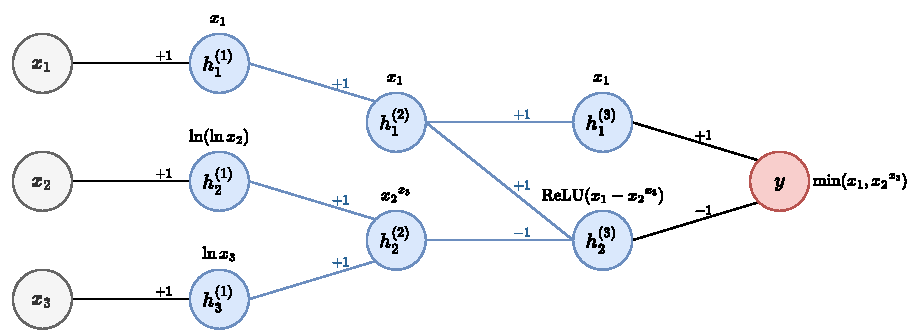
\includegraphics[width=0.9\textwidth]{assets/Q4_A_nn.pdf}
\end{figure}
و نورون‌ها نیز به این صورت می‌باشند:
\begin{LTR}
    \begin{table}[h]
        \centering
        \begin{tabular}{|c|c|c|c|c|}
            \hline
            \textbf{نورون} & \textbf{وزن‌ها}                                                    & \textbf{بایاس} & \textbf{فعال‌سازی تابع}        & \textbf{نهایی خروجی}                \\
            \hline \hline
            $h_1^{(1)}$    & $w_{11}^{(1)} = 1,\quad w_{21}^{(1)} = 0, \quad w_{31}^{(1)} = 0$ & $0$            & $\phi(z)=z$                   & $x_1$                               \\
            \hline
            $h_2^{(1)}$    & $w_{12}^{(1)} = 0,\quad w_{22}^{(1)} = 1,\quad w_{32}^{(1)} = 0$  & $0$            & $\phi(z)=\ln(\ln z)$          & $\ln(\ln x_2)$                      \\
            \hline
            $h_3^{(1)}$    & $w_{13}^{(1)} = 0,\quad w_{23}^{(1)} = 0,\quad w_{33}^{(1)} = 1$  & $0$            & $\phi(z)=\ln z$               & $\ln x_3$                           \\
            \hline \hline
            $h_1^{(2)}$    & $w_{11}^{(2)} = 1,\quad w_{21}^{(2)} = 0,\quad w_{31}^{(2)} = 0$  & $0$            & $\phi(z)=z$                   & $x_1$                               \\
            \hline
            $h_2^{(2)}$    & $w_{12}^{(2)} = 0,\quad w_{22}^{(2)} = 1,\quad w_{32}^{(2)} = 1$  & $0$            & $\phi(z)=e^{e^z}$             & $x_2^{x_3}$                         \\
            \hline \hline
            $h_1^{(3)}$    & $w_{11}^{(3)} = 1,\quad w_{21}^{(3)} = 0$                         & $0$            & $\phi(z)=z$                   & $x_1$                               \\
            \hline
            $h_2^{(3)}$    & $w_{12}^{(3)} = 1,\quad w_{22}^{(3)} = -1$                        & $0$            & $\phi(z)=\text{\lr{ReLU}}(z)$ & $\text{\lr{ReLU}}(x_1 - x_2^{x_3})$ \\
            \hline \hline
            $y$            & $w_{11}^{(y)} = 1,\quad w_{21}^{(y)} = -1$                        & $0$            & $\phi(z)=z$                   & $\min(x_1, x_2^{x_3})$              \\
            \hline
        \end{tabular}
    \end{table}
\end{LTR}

\item برای \lr{forward pass}، محاسبات را از گره‌های ورودی (فرزند) آغاز کرده و با حرکت به سمت راست، مقدار خروجی هر گره والد را بر اساس ورودی‌های آن محاسبه می‌کنیم تا در نهایت به خروجی سیستم ($f$) برسیم.

برای \lr{backward pass} نیز روند را برعکس کرده و از گره خروجی (ریشه) به سمت چپ حرکت می‌کنیم. در این مسیر، طبق قاعده‌ی زنجیره‌ای مشتق خروجی نسبت به هر متغیر را به دست می‌آوریم. به طور کلی اگر $z$ تابعی از $y$ و $y$ تابعی از $x$ باشد، طبق قاعده‌ی زنجیره‌ای داریم:
\begin{equation*}
    \frac{\partial z}{\partial x} = \frac{\partial z}{\partial y} \times \frac{\partial y}{\partial x}
\end{equation*}
بنابراین در الگوریتم \lr{forward pass}، ابتدا به مشتق خروجی نسبت به خودش مقدار $1$ را نسبت می‌دهیم ($\frac{\partial f}{\partial f} = 1$). سپس با حرکت به سمت چپ، مشتق نهاییِ گره‌ی فرزند برابر خواهد بود با حاصل‌ضرب مشتق نهایی گره‌ی والد در مشتق محلی خود تابع نسبت به آن ورودی (که روی یال‌ها مشخص شده است).

اگر مقادیر \lr{forward pass} را با رنگ آبی، مشتق‌های محلی هر تابع نسبت به ورودی‌هایش را با رنگ سبز و مشتق خروجی نهایی نسبت به هر گره را با رنگ قرمز نشان دهیم، گراف محاسباتی به همراه جزئیات گام‌به‌گام محاسبات به شکل زیر خواهد بود:

\begin{figure}[H]
    \centering
    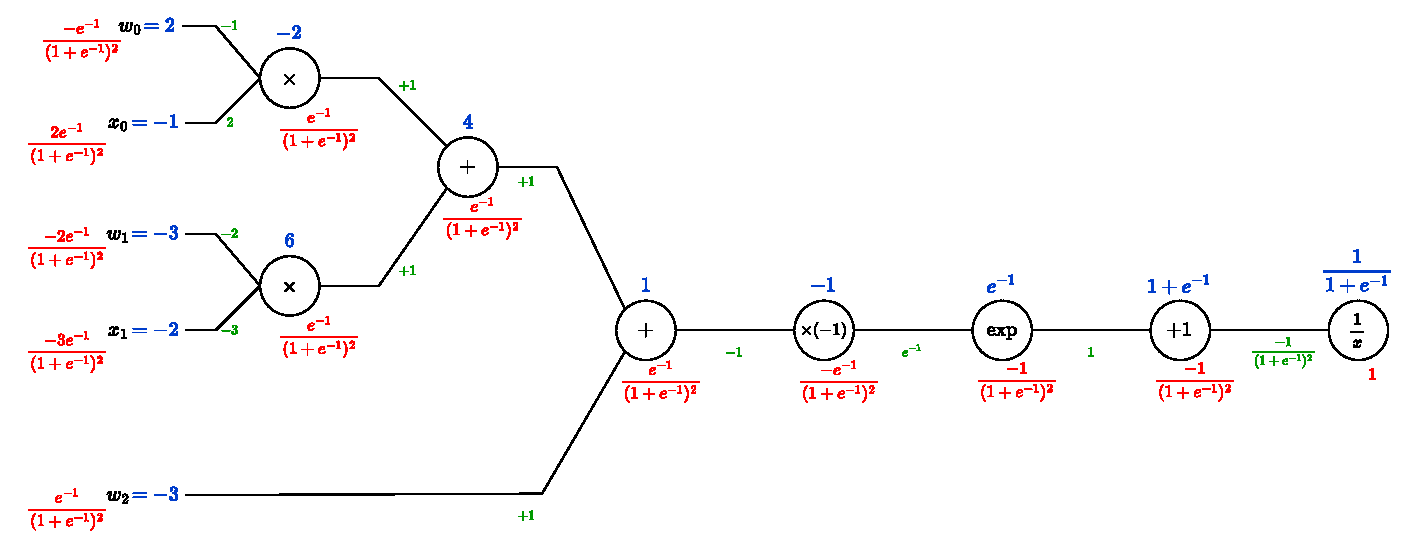
\includegraphics[width=1.0\textwidth]{assets/Q4_B_graph.pdf}
\end{figure}

خروجی گره‌های ضرب اول و دوم را به ترتیب با $v_1$ و $v_2$، خروجی اولین گره جمع را با $v_3$ و خروجی دومین گره جمع (قبل از اعمال علامت منفی) را با $v_4$ نام‌گذاری می‌کنیم. در نهایت، با اعمال قاعده‌ی زنجیره‌ای از راست به چپ، مشتق خروجی نهایی نسبت به تک‌تک پارامترها و وزن‌های ورودی به صورت زیر محاسبه می‌شود:
\begin{align*}
    \frac{\partial f}{\partial w_0} & = \frac{\partial f}{\partial v_1} \times \frac{\partial v_1}{\partial w_0} = \frac{e^{-1}}{(1+e^{-1})^2} \times x_0 = \frac{-e^{-1}}{(1+e^{-1})^2} \approx -0.197  \\
    \frac{\partial f}{\partial x_0} & = \frac{\partial f}{\partial v_1} \times \frac{\partial v_1}{\partial x_0} = \frac{e^{-1}}{(1+e^{-1})^2} \times w_0 = \frac{2e^{-1}}{(1+e^{-1})^2} \approx 0.393   \\
    \frac{\partial f}{\partial w_1} & = \frac{\partial f}{\partial v_2} \times \frac{\partial v_2}{\partial w_1} = \frac{e^{-1}}{(1+e^{-1})^2} \times x_1 = \frac{-2e^{-1}}{(1+e^{-1})^2} \approx -0.393 \\
    \frac{\partial f}{\partial x_1} & = \frac{\partial f}{\partial v_2} \times \frac{\partial v_2}{\partial x_1} = \frac{e^{-1}}{(1+e^{-1})^2} \times w_1 = \frac{-3e^{-1}}{(1+e^{-1})^2} \approx -0.590 \\
    \frac{\partial f}{\partial w_2} & = \frac{\partial f}{\partial v_4} \times \frac{\partial v_4}{\partial w_2} = \frac{e^{-1}}{(1+e^{-1})^2} \times 1 = \frac{e^{-1}}{(1+e^{-1})^2} \approx 0.197
\end{align*}

\end{ابجد}